%!TEX root = ../Thesis.tex
\section{Beschreibung des Projektverlaufs}

\subsection{Tatsächliche Aufgabenverteilung im Team (tabellarisch)}

\pagebreak

\subsection{Teammeeting-Protokolle}

{\def\arraystretch{1.5}\tabcolsep=5pt
\begin{longtable}{|l|l|p{11cm}|}
	\hline
	\textbf{Datum} & \textbf{Dauer} & \textbf{Beschreibung}
	\\ \hline \hline
	\endfirsthead
	
	\hline
	\multicolumn{3}{|c|}{\textit{...Forsetzung der Tabelle}}
	\\ \hline \hline
	\textbf{Datum} & \textbf{Dauer} & \textbf{Beschreibung}
	\\ \hline \hline
	\endhead
	
	\hline \hline
	\multicolumn{3}{|c|}{\textit{Tabelle wird auf der nächsten Seite fortgesetzt...}}
	\\ \hline
	\endfoot
	
	\hline \hline
	% 1210 Minuten
	\multicolumn{3}{|c|}{\textit{Summe der Dauer aller Meetings beträgt 21 Stunden}}
	\\ \hline
	\endlastfoot
	
		\textbf{03.09.2019} & \textbf{200 Min.} &
			\textbf{\#1}
			\\ & &
			Auswahl des Projekttyps. Entscheidung für die Entwicklung einer Android-App.
			\\ & &
			Erste Einarbeitung in die Thematik. Lesen des bereitgestellten Dokuments mit Aufgabenstellung, groben Anforderungen und weiteres. 
			\\ & &
			Konzepterarbeitung auf Papier. Vorstellung und Diskussion verschiedener Ansätze.
	\\\hline
		\textbf{04.09.2019} & \textbf{110 Min.} &
			\textbf{\#2}
			\\ & &
			Einigung mit dem Dozenten auf einen Ansatz für den Taschenrechner.
			\\ & &
			Workflow für Git, Meeting-Protokolle, Studienarbeit und Projekttagebücher festlegen.
			\\ & &
			Ausarbeitung des Konzepts für den Taschenrechner. Hier wurden dem Auftraggeber Herr Seifert mehrere Konzepte vorgestellt und gemeinsam mit ihm genaue Anforderungen erarbeitet.
	\\\hline
		\textbf{05.09.2019} & \textbf{20 Min.} &
			\textbf{\#3}
			\\ & &
			Fertigstellung des Konzeptes.
			\\ & &
			Fortschritte beim Paper-Prototypen.
			\\ & &
			Android-Umgebung ist bei allen Team-Mitgliedern komplett aufgesetzt und lauffähig.
	\\ \cline{2-3}
		& \textbf{60 Min.} &
			Besprechung des aktuellen Stands des Konzepts und des Prototypen.
			\\ & &
			Erstellung eines Mid-Fidelity Prototypen.
			\\ & &
			Diskussion über Umsetzung und Workflow der App.
			\begin{itemize}\renewcommand\labelitemi{--}
				\item  Wie sollen die einzelnen Kacheln funktionieren?
				\item Wie sollen die Kacheln miteinander interagieren?
				\item Wie könnte die Architektur der App aussehen?
			\end{itemize}
	\\ \cline{2-3}
		& \textbf{40 Min.} &
			Projektplanung mithilfe von Projektstrukturplan und weiteren Methoden.
			\\ & &
			Übertragen der Ergebnisse in den Teams-Planner.
			\\ & &
			Grobe Verteilung der Arbeitspakete innerhalb des Teams.
	\\\hline
		\textbf{17.09.2019} & \textbf{ 60 Min.} &
			\textbf{\#4}
			\\ & &
			Erweiterung UML-Klassendiagramm. Die Klasse Operand wird abstrakt und wird von konkreten Operanden wie Vector geerbt. Diese stellen Extensions dar die neben den eigentlichen mathematischen Werten weitere Daten und Verhalten mitbringen.
			\\ & &
			Welche Library soll für Mathe-Funktionalitäten benutzt werden? JScience und die bereits mitgelieferte Standardbibliothek.
	\\\hline
		& \textbf{90 Min.} &
			Wie sollen Elemente in der GUI dargestellt werden? Als Character oder gerendert in LaTeX. Letzteres ist mit höherer Komplexität verbunden sieht aber auch besser aus. 
			\\ & &
			Wie soll das Layout funktionieren? Gridlayout fällt raus, weil nicht dynamisch genug? Relative-Layout ist eine Option. Hier darf aber die Anordnung beim Rotieren nicht unkontrolliert verändert werden. UI Team möchte, dass alle Komponenten gleich groß sind. In dem Fall kann man Gridlayout benutzen.
			\\ & &
			Wie soll die Eingabe von Funktionen im Graph Operand funktionieren? Nur möglich mit bereits vorhandenen Elementen in der Oberfläche. Es öffnet sich keine Tastatur.
	\\\hline
		\textbf{09.10.2019} & \textbf{90 Min.} &
			\textbf{\#5}
			\\ & &
			Vorstellung des Backend-Entwurfs für Teammitglieder, die für das Frontend zuständig sind.
			\\ & &
			Vorstellung des Frontend-Entwurfs für Teammitglieder, die für das Backend zuständig sind.
			\\ & &
			Diskussion über Verbindung von Frontend und Backend. Wie abgekoppelt lässt sich der Calculator wirklich realisieren?
			\\ & &
			Vorstellung der Hauptbibliothek die für die (aufwändigen) Rechnungen wie Nullstellenberechnung benutzt werden soll.
			\\ & &
			Warum Apache Commons Math und nicht JScience?
			\\ & &
			Diskussion des Programm-Workflows.
	\\ \hline
		\textbf{05.01.2020} & \textbf{120 Min.} &
			\textbf{\#6}
			\\ & &
			Aufnahme des aktuellen Projektstands.
			\\ & &
			Besprechung des weiteren Vorgehens.
			\\ & &
			Aufgabenabstimmung.
			\\ & &
			Besprechung des geplanten Frontends.
			\\ & &
			Besprechung/ Lösung von Problemen.
	\\ \hline
		\textbf{14.01.2019} & \textbf{90 Min.} &
			\textbf{\#7}
			\\ & &
			Zusammenführung Frontend Backend
			\\ & &
			Präsentation des Frontends durch das GUI-Team.
			\\ & &
			Besprechen von MVC-Umsetzung in Android.
			\\ & &
			Backend Unit-Testing Fortschritte.
			\\ & &
			Serialisierung der Stacks zur Session-Sicherung.
	\\ \hline
		\textbf{24.01.2019} & \textbf{240 Min.} &
			\textbf{\#8}
			\\ & &
			Detaillierte Ausarbeitung der Architektur im Backend.
			\\ & &
			Programmieren im Team. 
			\\ & &
			Zusammenführen mehrere Features.
			\\ & &
			Umbau der Programmstruktur.
	\\ \hline
		\textbf{28.01.2019} & \textbf{90 Min.} &
			\textbf{\#9}
			\\ & &
			Gespräch mit Herr Prof. Dr. Thomas Seifert über den aktuellen Stand des Projekts und im Anschluss daran eine Nachbesprechung innerhalb des Teams.
			\\ & &
			Vorstellung:
			\begin{itemize}\renewcommand\labelitemi{--}
				\item Vorstellung der bereits implementierten Grundfunktionen der App.
				\item Vorstellung des verwendeten Design-Patterns.
				\item Abgleich von Umsetzung mit den Anforderungen des Dozenten.
				\item Ansatz des Backends erklärt.
				\item Gerät ausleihen, um nicht nur mit Emulator testen zu können.
				\item Serialisierung der Daten (Speichern und Laden).
			\end{itemize}
			\\ & &
			Ergebnis:
			\begin{itemize}\renewcommand\labelitemi{--}
				\item Projekt ist auf einem guten Weg. Priorisiert werden sollen differenzierende Funktionen anstatt wenige Features sehr detailliert auszuarbeiten (Prototypische Arbeit).
				\item Ternäre, Quaternäre usw. Operationen sind gewünscht.
				\item Vektoren in Bestandteile lösen.
				\item Eingabe von Matrizen.
				\item Jeder Klasse muss ein Verantwortlicher zugeordnet sein.
			\end{itemize}
			\\ & &
			Ideen aus der Nachbesprechung:

			\begin{itemize}\renewcommand\labelitemi{--}
				\item ''Vektor bauen'' / ''Vektoren auflösen'' Action. 
				\item Summe von Stack Action.
				\item 1x Triple Operator einfügen.
				\item Operanden Eingabe via einzelne Menüs.
				\item Ranks der Stacks anpassen.
				\item Format des ersten Stacks anpassen.
			\end{itemize}
	\\ \hline
		\textbf{03.02.2019} & \textbf{90 Min.} &
			\textbf{\#10}
			\\ & &
			Besprechen des aktuellen Stands der App.
			\\ & &
			Was muss noch unbedingt umgesetzt werden?
			\\ & &
			Aufteilung der noch offenen Kapitel in der Ausarbeitung.
			\\ & &
			Neues Kapitel ''Einleitung'' mit Motivation.
			\\ & &
			Anpassung einiger Kapitelbezeichnungen an Gegebenheiten des Projekts.
			\\ & &
			Koordination der Ausarbeitung.
	\\
\end{longtable}
}

\subsection{Projekttagebücher}

\subsubsection{Tom Bockhorn}

\subsubsection{Hendrik Falk}

\subsubsection{Dennis Gentges}

\subsubsection{Getuart Istogu}

\subsubsection{Jannis Keienburg}

\subsubsection{Tim Jonas Meinerzhagen}

\subsubsection{Khang Pham}

\subsubsection{Tim Schwenke}

\subsection{Beschreibung von Problemen}

\subsubsection{Softwareentwicklung im Team [Schwenke]}

Schon kurz nach der initialen Erstellung des Git-Repositories und des Projekts in Android-Studio hat sich die Frage gestellt, wie man in einem acht Mitglieder starkem Team produktiv an einer einzelnen Code-Basis arbeiten soll. Hat man ein Quellcodeverzeichnis alleine für sich reichen zumeist um die drei aktive (also nicht \textit{stale}) Branches aus. Das wäre zunächst der \code{Master}-Branche, welcher die Wurzel des Verzeichnisses darstellt und – gerade, wenn Ansätze wie CI/CD verfolgt werden – die produktiven oder zumindest lauffähigen Versionen eines Projekts enthält. Im \code{Development}-Branch hingegen findet die Entwicklung statt. Hier ist es üblich, dass das Projekt zum Zeitpunkt einzelner Commits Fehler enthält und nicht lauffähig ist. Sobald ein Entwickler der Meinung ist, dass der Stand in \code{Development} veröffentlicht werden kann, wird \code{Development} in \code{Master} vereint. Wichtig zu betonen ist hier, dass dies keine feste Regel ist, sondern eher dem allgemeinen Workflow entspricht. In einem großen Team ist ein solcher Arbeitsablauf nicht mehr möglich. So müssen mehrere Entwickler parallel an dem Projekt arbeiten. Verwendet man nun das System aus zwei Branches, wird es sehr schnell zu Merge-Konflikten kommen, die die Entwickle dazu zwingen sich mehr mit der korrekten Zusammenführung als der eigentlichen Entwicklung zu beschäftigen, sofern sie ihren lokalen Arbeitsbereich aktuell halten wollen. Die nächstliegende und ebenfalls problematische Alternative ist es nur bei Fertigstellung von Funktionen, die meist aus mehreren Commits zusammengesetzt sind, das lokale Quellcodeverzeichnis mit dem Remote zu synchronisieren. Mit dieser Herangehensweise verpasst man unter Umständen große Fortschritte im Gesamtprojekt. Die lokale Version ist plötzlich nicht mehr lauffähig und muss aufwändig angepasst werden. Deswegen wird im Rahmen dieses Projekts der\textit{ Gitflow-Workflow} verwendet. Grafisch dargestellt ist dieser beispielhaft in der folgenden Grafik.

\begin{figure}[h]
	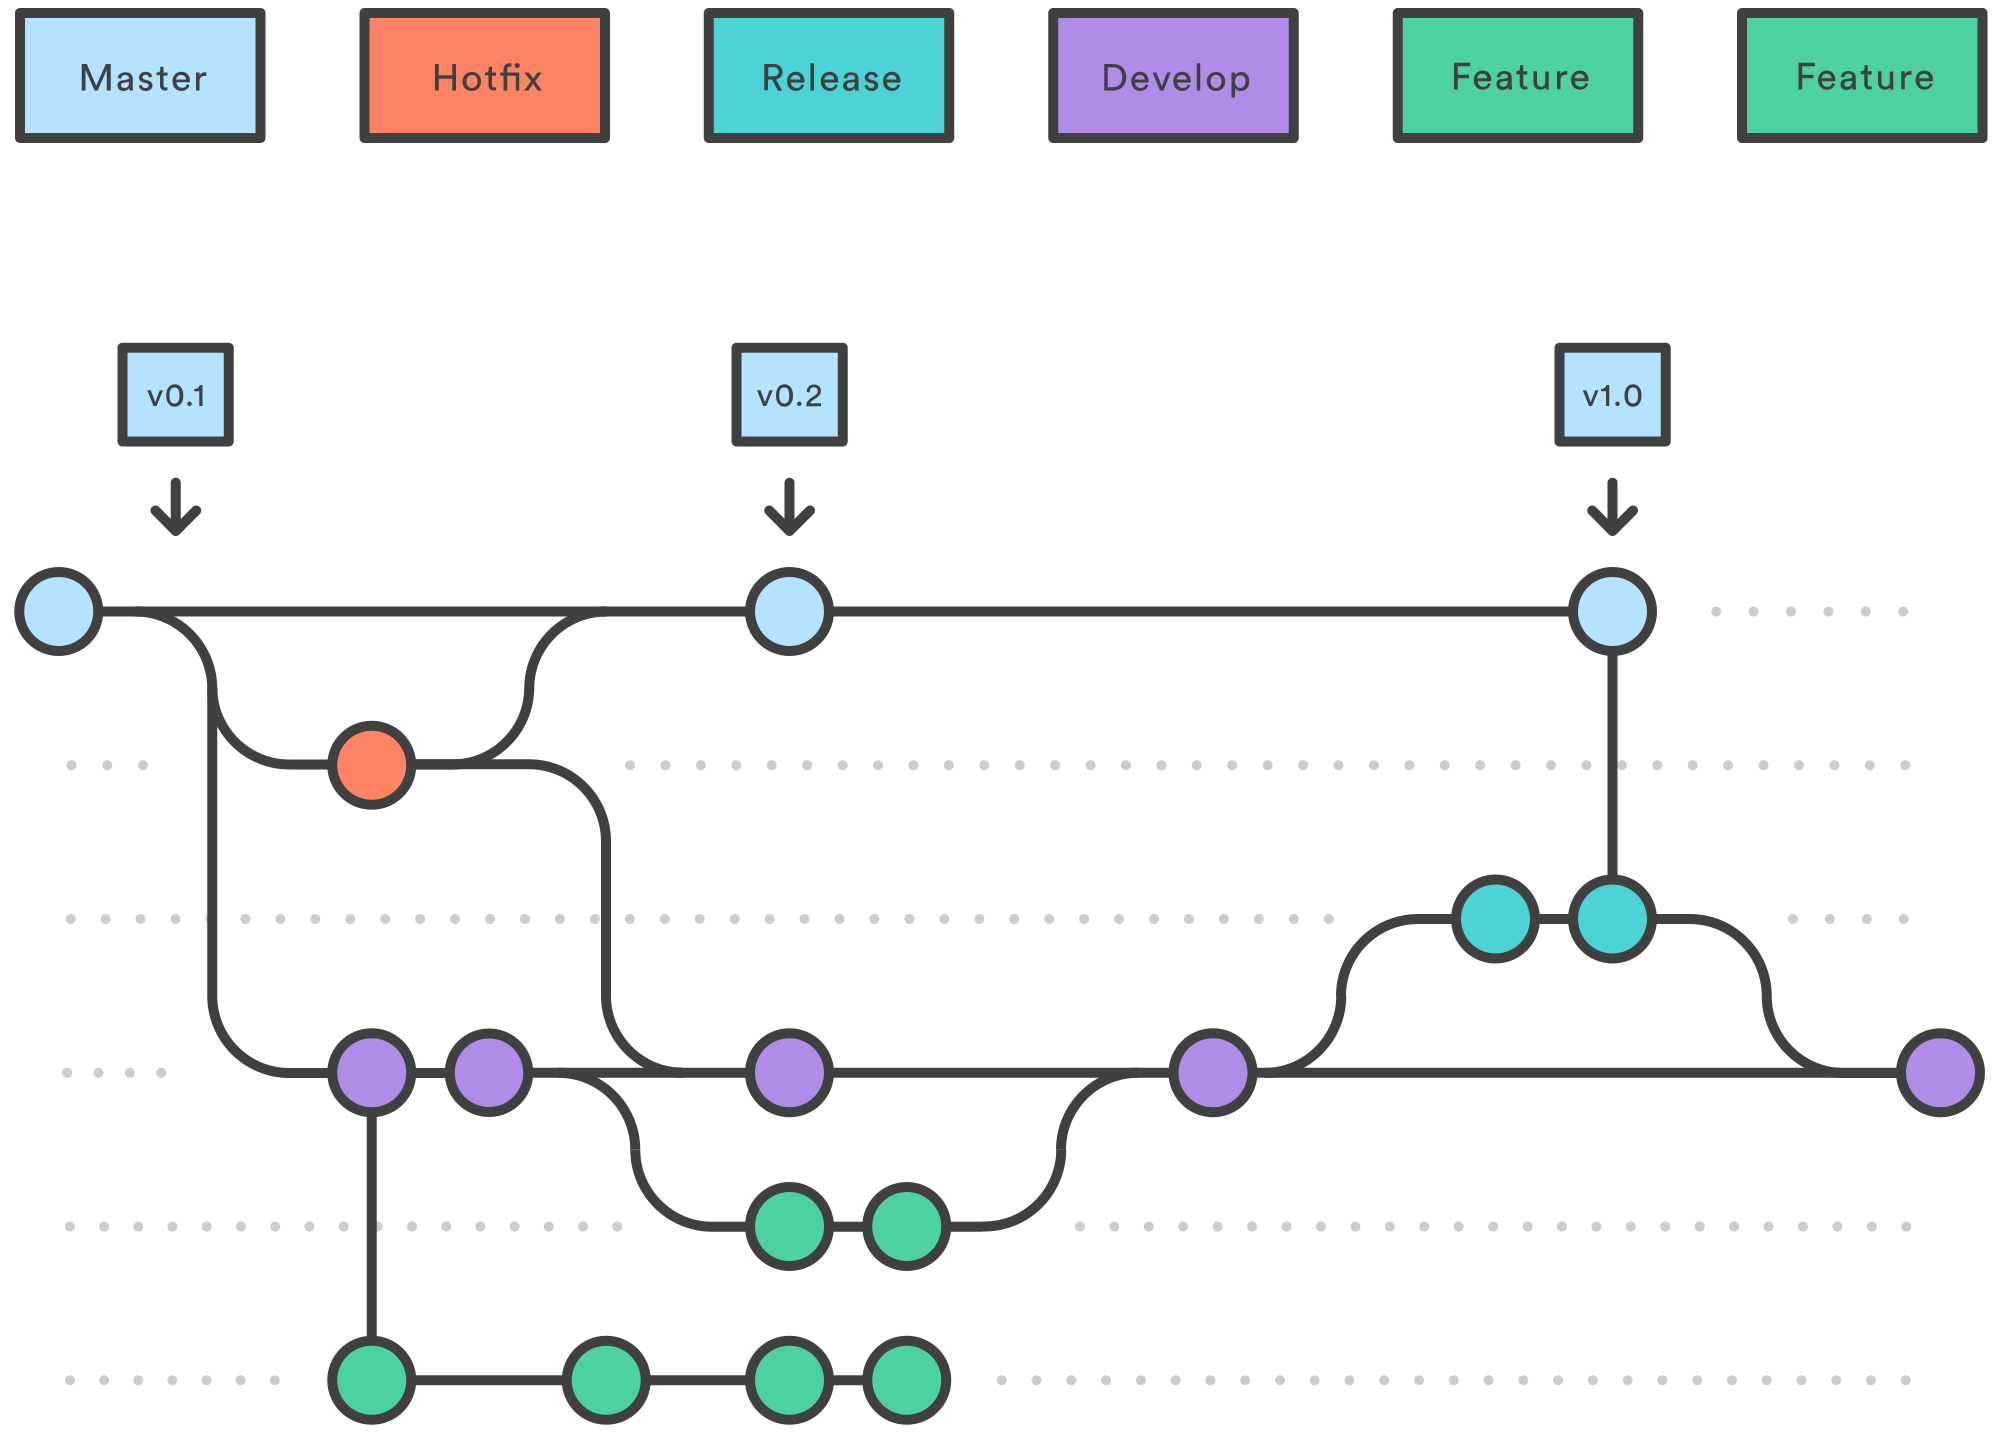
\includegraphics[width=\columnwidth]{img/gitflow}
	\caption[Gitflow]{Gitflow\footnotemark}
\end{figure}
\footnotetext{\cite{atlassian2020}}

Der Gitflow-Workflow definiert ein strenges Branching-Model und gibt jedem Typ von Branch (lediglich differenziert durch ihre Namen) eine spezifische Rolle. \code{Master} wird verwendet, um die Release-History festzuhalten. Hier finden sich Versionen des Projekts, die lauffähig sind und für sich alleine stehen (können). \code{Development} fungiert ähnlich wie \code{Master}, nur enthält es die gesamte Entwicklungshistorie des Projekts. Nun kommen die sogenannten \code{Feature}-Branches ins Spiel. Benannt werden Features hierarchisch. Im Projekt werden folgende zwei Gruppen verwendet: 

\begin{minipage}{\textwidth}
\texttt{feature/\textbf{backend}/<konkretes-feature>}

\texttt{feature/\textbf{frontend}/<konkretes-feature>}
\end{minipage}

Jedes Feature wird einem Verantwortlichen zugeteilt und wird meist auch von diesem bearbeitet. Sobald ein Feature fertig ist, wird es in \code{Development} zusammengeführt. Somit werden die Abstände zwischen Zusammenführungen verringert und der Arbeitsablauf wird einfacher. Schließlich gibt es auch noch einen Hotfix-Branch für dringende Änderungen.

Im Laufe der Entwicklung haben sich die Vorteile dieser Herangehensweise für das Team deutlich gezeigt. Unterschiedliche Features konnten, nachdem eine grundlegende Programmarchitektur umgesetzt worden ist, meist ohne Probleme zusammengeführt werden. 